\subsection*{Overall comments} % todo

\RC{} This study proposed an integrated index that incorporates water resources, water use, and water allocation to represent the water governance regime in the Yellow River basin. The authors showed an in-depth understanding of the water governance in this basin and made a great effort to represent the status of water governance straightforwardly with the integrated index. The figures were generally well-designed and presented clearly. But I feel the paper lacks details of the results which makes it difficult to understand the paper. Specific comments are listed below.

% 感谢您认可。
% 很抱歉缺少细节,可能会使您难以完全理解我们的研究。
% 为了回应您的担忧,我们已经修改了我们的稿件,并提供了更详细的结果解释。请在下面找到我们对您的具体评论的逐条回复。
\AR{} Thank you for your valuable feedback and for acknowledging our efforts in understanding the water governance in the Yellow River basin. We appreciate your comments regarding the clarity of the figures and our integrated index. Sorry about the lack of details in the results section may have made it difficult to fully comprehend our study. In response to your concerns, we have revised our manuscript and provided a more detailed explanation of the results. Please find our point-by-point response to your specific comments below.

\subsection{Major concern \#1}

% 气候变化在指数中没有明确的体现,这可能是本世纪黄河流量恢复的关键因素。气候变化将是未来该流域面临的巨大挑战。重大的气候变化可能影响流域的适应能力,因此需要不同的治理策略。
\RC{} Climate change is not explicitly represented in the index, which might play a key role in the streamflow recovery in the Yellow River in this century. Climate change would be a great challenge in the basin in the future. Significant climate change may affect the adaptive capacity of a basin and thus require different governance strategies.

% 气候变化的确会产生很多影响,例如改变降水量和蒸发量。但这些影响都会以影响可用水量的形式体现在IWGI之中。
% 在新增加的图表中,我增加了天然水量的图表展示这种变化
% 例如气候变化让可用水量发生改变(scarcity),极端气候让我们难以有效的分配水资源(allocation),对气候变化的适应可能导致社会变革,让人们对愈发侧重于工业和经济发展的治理策略进行反思(priority)。
% 我们现在在讨论中涉及了这些话题。
\AR{} Climate change indeed has a multitude of impacts, such as altering precipitation and evaporation rates.
However, these effects are inherently captured within the Integrated Water Governance Index (IWGI) as they influence the available water resources.
In the revised version of our paper, we have added new graphs to demonstrate the changes in natural water availability caused by climate change.
For example, climate change may alter water scarcity levels and make it more difficult to effectively allocate water resources due to extreme climate events.
Additionally, adapting to climate change could lead to societal transformations, prompting a reevaluation of governance strategies that increasingly focus on industrial and economic development (priority).
We have now addressed these topics in our discussion, illustrating the various ways in which climate change influences the adaptive capacity of a basin and its subsequent governance requirements.

\begin{quote}[page=3, sline=83, eline=88]
	\DIFadd{An important reason for developing this new index is practices of water governance changes throughout development under a hybrid of social and natural drivers.
	First, besides climate change impacts embedded in current water yield concerns, water stress is also tightly related to an }\DIFaddend increasingly insatiable demands from economic activities\DIFdelbegin \DIFdel{such as irrigation and industry; water storage can resolve some but not all of these issues
	}\DIFdelend \DIFaddbegin \DIFadd{, while developing water storage to release the stress~}\DIFaddend~\cite{qin2019,wada2014,huang2021}.
\end{quote}

\begin{figure}[!htb]
	\centering
	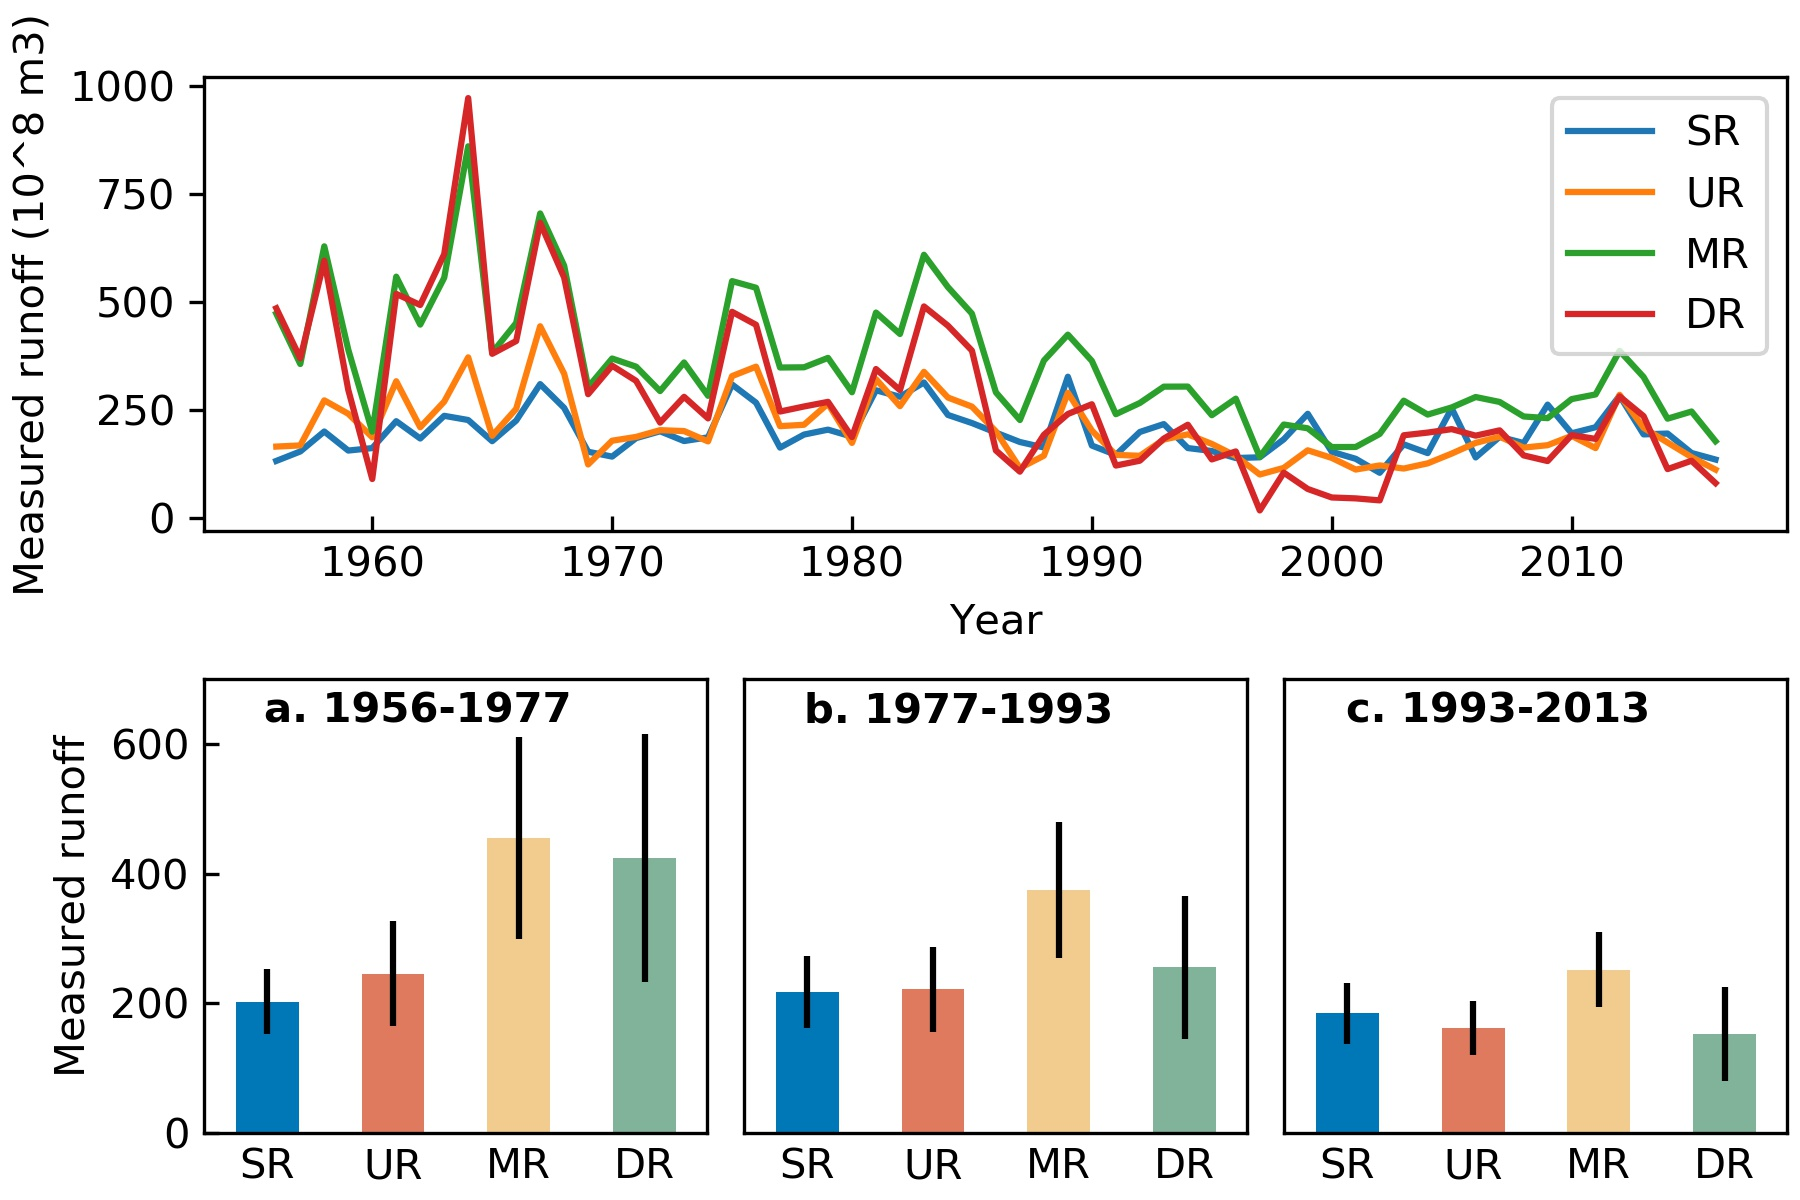
\includegraphics[width=\textwidth]{sup/sf_measured_runoff.jpg}
	\caption{绘图测试}\label{fig:xfig0}
\end{figure}

% 我们强调流域治理需要考虑这些因素,但我们可能很难穷尽优秀的流域治理策略需要考虑哪些因素。因此,IWGI至少让我们可以知道在诸多治理因素的共同影响下,流域的未来正在走向何方。
\AR*{}

\subsection{Major concern \#2}
% 结果是总结性的。我建议提供更多关于三个指数和IWGI结果的信息。例如,三个指标的结果,以及分区域的结果。请解释IS、IP、IA和IWGI这三个指标的范围,以及不同数值的含义。这些细节可以帮助读者理解结果的合理性。
\RC{} The results are summative. I would suggest providing more information on the results of the three indices and the IWGI.\ For example, the results of the three indices, and the results for the sub-regions. And please explain the range of the three indicators, IS, IP, IA, and the IWGI, and the meanings of different values. These details could help readers understand the reasonability of the results.

% 感谢您指出这一点,非常抱歉过于总结性的手稿带来的困惑。
% 在新的手稿中,我们将各指数的情况总结到补充材料,并在正文中对有关各指数情况的图表总结。
% 在方法中,我们补充了指标的取值范围(三个子指标的变化范围都是0~1)。
\AR{} Thank you for pointing this out, and we apologize for the confusion caused by the overly conclusive manuscript. In the revised manuscript, we have summarized the indicators by graphs with description in supplementary material:in the supplementary material.

% TODO 这里记得写一下是哪几个附图
\AR*{} Figure SX to SX are three indicators changing trends with different regions' contribution.

\AR*{} In the method, we added the value range of the index. Ranges of three indicators and meaning of their values are further explained in the methodology section, now:

\begin{quote}[page=1, sline=1]
	Methods
\end{quote}

\subsection{Major concern \#3}
% 本研究中使用的数据似乎有不同的时间段,大多数数据来自2013年之前。近十年来,黄河的水文状况和水治理应该发生了重大变化。因此,结合近十年的结果将使这项研究更加可靠。
\RC{} The data used in this study seem to have different time periods, and most data are from before 2013. The hydrological regime and water governance in the Yellow River should have changed significantly in the recent decade. Therefore, incorporating the result from the recent decade would make this study more solid.

\AR{} Multiple-source dataset.

\subsection{Major concern \#4}
% 这三个指标之间可能存在相互作用/相互联系。作者是否检查了指标之间的关系?
\RC{} There might be interactions/interconnections among the three indicators. Did the authors examine the relations between the indicators?

\AR{} Yes, we did examination for the interconnections between the three indicators. Sorry we didn't make the information accessible. Now, we added a table to describe them:

\begin{quote}
	Table
\end{quote}

\AR*{} Note that independent is not required in our approach, as three aspects are intertwined in essence (we explained this in the introduction).
However, our

\subsection{Major concern \#5}
% IWGI在“应力”方面包含储层存储信息。输水能力是衡量水治理/水社会复原力的重要指标。
\RC{} The IWGI includes reservoir storage information in the "stress" aspect. However, the water conveyance ability is not represented, which is also an important indicator of water governance/hydrosocial resilience.

% 短期的输水能力是衡量水治理/水社会复原力的重要指标
% 但年尺度上,变化不大
\AR*{} Correct, conveyance is crucial to water governance/water society resilience, especially in the short term. However, the IWGI in this study focuses on annual time resolution. At this scale, conveyance has a less significant impact on water governance. From this point of view, we have two reasons that IWGI doesn't have to consider this in our study:

% 我们检验过了年尺度的输水数据,基本变化不大

% 水治理很复杂,考虑到越来越多的要素会增加其复杂度。Scarcity是本研究使用最复杂的指标,因为这是一个经过检验的,可以有效表征的指数。如果经过检验影响不大,没有必要增加复杂度。

\subsection{Major concern \#6}
% 我建议在标题中加上“黄河流域”。因为没有对IWGI的适用性和有效性进行测试或讨论。它能在其他盆地使用吗?使用索引的先决条件是什么?
\RC{} I would suggest adding "Yellow River basin" in the title. Because the applicability and validity of the IWGI were not tested or discussed. Can it be used in other basins? What is the prerequisite for using the index?

% 感谢你的提议,我们增加了黄河流域

% 关于IWGI的泛用性,实际上我们在讨论中讨论了这一点。我们也

% 我们如今在方法部分提到了使用它的先决条件。

\subsection{Major concern \#7}
% 最好在引言部分解释“水治理机制”的概念,然后解释使用综合指数IWGI代表水治理机制的必要性。
\RC{} It would be better to explain the concept "water governance regime" in Introduction and then explain the necessity of using the integrated index IWGI for representing the water governance regime.

% 感谢你的建议,我们做了如下解释:
\begin{quote}
	``Water governance regime'' is \ldots
\end{quote}

\subsection{Detailed issues}

% 我没有在引用的文献中找到“用水的三个核心方面”。这三个方面是作者提出的吗?
\RC{} Line 57-62: I did not find the "three core aspects of water use" in the cited reference. Were the three aspects put forward by the authors?

\RC{} Line 92: missing information for the citation?

\RC{} Line 94-95: the sentence is unclear.

\RC{} Line 121: Repeated citation Qin et al. 2019.

\RC{} Line 122: It would be better to introduce the calculation of SFV in the main text.

\RC{} Equation (6): Why is the numerator WUpro not WUnon-pro? Please check the equation.

\RC{} Equation (7): CEM => AEM?

\RC{} Line 154: Please explain the source of irrigated area data.

\RC{} Fig.2A, p<0.01 or p<0.001? (line 147 says that α=0.001 was used for the change-point detection).

\RC{} Fig.2C: How were the directions determined?

\RC{} Fig.3C: What do the dashed lines denote?

\RC{} Line 187: what is "social transformation"?

\RC{} Line 208: the IWGI was proposed in this study, here the citations of Loch's and Turton's studies are not appropriate.

\RC{} Line 273: adapted => adopted?

\RC{} Line 275: biophysical? Please check the sentence.

\AR{} \dots
